\documentclass{beamer}
\mode<presentation>
\usepackage{amsmath}
\usepackage{amssymb}
%\usepackage{advdate}
\usepackage{adjustbox}
\usepackage{subcaption}
\usepackage{enumitem}
\usepackage{multicol}
\usepackage{mathtools}
\usepackage{listings}
\usepackage{url}
\usepackage{tikz}
\usetikzlibrary{matrix, calc}
\def\UrlBreaks{\do\/\do-}
\usetheme{metropolis}
%\usecolortheme{lily}
\setbeamertemplate{footline}
{
	\leavevmode%
	\hbox{%
		\begin{beamercolorbox}[wd=\paperwidth,ht=2.25ex,dp=1ex,right]{author in head/foot}%
			\insertframenumber{} / \inserttotalframenumber\hspace*{2ex} 
		\end{beamercolorbox}}%
		\vskip0pt%
	}
	\setbeamertemplate{navigation symbols}{}

	\providecommand{\nCr}[2]{\,^{#1}C_{#2}} % nCr
	\providecommand{\nPr}[2]{\,^{#1}P_{#2}} % nPr
	\providecommand{\mbf}{\mathbf}
	\providecommand{\pr}[1]{\ensuremath{\Pr\left(#1\right)}}
	\providecommand{\qfunc}[1]{\ensuremath{Q\left(#1\right)}}
	\providecommand{\sbrak}[1]{\ensuremath{{}\left[#1\right]}}
	\providecommand{\lsbrak}[1]{\ensuremath{{}\left[#1\right.}}
	\providecommand{\rsbrak}[1]{\ensuremath{{}\left.#1\right]}}
	\providecommand{\brak}[1]{\ensuremath{\left(#1\right)}}
	\providecommand{\lbrak}[1]{\ensuremath{\left(#1\right.}}
	\providecommand{\rbrak}[1]{\ensuremath{\left.#1\right)}}
	\providecommand{\cbrak}[1]{\ensuremath{\left\{#1\right\}}}
	\providecommand{\lcbrak}[1]{\ensuremath{\left\{#1\right.}}
	\providecommand{\rcbrak}[1]{\ensuremath{\left.#1\right\}}}
	\theoremstyle{remark}
	\newtheorem{rem}{Remark}
	\newcommand{\sgn}{\mathop{\mathrm{sgn}}}
	\providecommand{\abs}[1]{\left\vert#1\right\vert}
	\providecommand{\res}[1]{\Res\displaylimits_{#1}} 
	\providecommand{\norm}[1]{\lVert#1\rVert}
	\providecommand{\mtx}[1]{\mathbf{#1}}
	\providecommand{\mean}[1]{E\left[ #1 \right]}
	\providecommand{\fourier}{\overset{\mathcal{F}}{ \rightleftharpoons}}
	%\providecommand{\hilbert}{\overset{\mathcal{H}}{ \rightleftharpoons}}
	\providecommand{\system}{\overset{\mathcal{H}}{ \longleftrightarrow}}
	%\newcommand{\solution}[2]{\textbf{Solution:}{#1}}
	%\newcommand{\solution}{\noindent \textbf{Solution: }}
	\providecommand{\dec}[2]{\ensuremath{\overset{#1}{\underset{#2}{\gtrless}}}}
	\newcommand{\myvec}[1]{\ensuremath{\begin{pmatrix}#1\end{pmatrix}}}
		\let\vec\mathbf

		\lstset{
			%language=C,
			frame=single, 
			breaklines=true,
			columns=fullflexible
		}

		\numberwithin{equation}{section}

		\title{Sprog Presentation}
		\author{Akshara Sarma Chennubhatla,\\ EE24BTECH11003,\\IIT Hyderabad.\\}

		\date{\today} 
		\begin{document}

		\begin{frame}
			\titlepage
		\end{frame}

		\begin{frame}
			\frametitle{Problem Statement}
A train travels $360km$ at a uniform speed. If the speed had been $5km/h$ more, it would have taken $1$ hour less for the same journey. Find the speed of the train.
		\end{frame}
		\subsection{Solution}
		\begin{frame}
      \frametitle{Theoretical Solution}
		Let $s$ be the speed of the train, then,
\begin{align}
	\frac{360}{s} - 1 &= \frac{360}{s + 5}\\
	\implies s^2 + 5s &= 1800
\end{align}
Using the quadratic formula,
\begin{align}
	s &= \frac{-5 \pm \sqrt{5^2 - 4\brak{1}\brak{-1800}}}{2\brak{1}}\\
	s &= -45, 40
\end{align}
\end{frame}
\begin{frame}
      \frametitle{Simulated Solution - 1}
	By Newton-Ralphson method,\\
Take initial guess $s_0$, then run the following loop,
\begin{align}
	s_{n+1} &= s_n - \frac{f\brak{s_n}}{f^\prime\brak{s_n}}\\
	f\brak{s} &= s^2 + 5s - 1800\\
	f^\prime\brak{s} &= 2s + 5\\
	s_{n+1} &= s_n - \frac{s_n^2 + 5s_n - 1800}{2s_n + 5}
\end{align}
\end{frame}
		\begin{frame}
      \frametitle{Simulated Solution - 1}
The values of $s$ got through this method are,
\begin{align}
	s &= -45\\
	s &= 40
\end{align}
\end{frame}
\begin{frame}
      \frametitle{Simulated Solution - 2}
			Alternatively, we can solve the question by using the eigen values of the companion matrix.\\
For a polynomial equation of form $x_n+c_{n-1}x^{n-1}+\dots+c_2x^2+c_1x+c_0 = 0$ the companion matrix if of the form
\begin{align}
	\myvec{
		0 & 0 & \cdots & 0 & -c_0\\
		1 & 0 & \cdots & 0 & -c_1\\
		0 & 1 & \cdots & 0 & -c_2\\
		\vdots & \vdots & \ddots & \vdots & \vdots\\
		0 & 0 & \cdots & 1 & -c_{n-1}\\
	}
\end{align}
\end{frame}
\begin{frame}
      \frametitle{Simulated Solution - 2}

The eigen values of this matrix are the roots of the polynomial equation. For this question,
\begin{align}
	n &= 2\\
	c_0 &= -1800\\
	c_1 &= 5\\
	C &= \myvec{0 & 1800 \\ 1 & -5}
\end{align}
\end{frame}
\begin{frame}
	\frametitle{Simulated Solution - 2}
	To find the eigen values of the matrix, we use the method of $QR$ decomposition of the matrix.\\
The $QR$ algorithm decomposes a matrix $A$ into the product of an orthogonal matrix $Q$ and an upper triangular matrix $R$, such that
\begin{align}
	A = QR
\end{align}
The matrix is then updated iteratively as:
\begin{align}
	A_{new} = RQ
\end{align}
This process is repeated until $A$ converges to an upper triangular form.\\
\end{frame}

\begin{frame}
	\frametitle{Simulated Solution - 2}
	A square matrix A of order $n \times n$ is said to be in upper Hessenberg form if all the entries below the first subdiagonal are zero.
For example:
\begin{align}
	H = 
	\begin{bmatrix}
		h_{11} & h_{12} & h_{13} & \cdots & h_{1n} \\
		h_{21} & h_{22} & h_{23} & \cdots & h_{2n} \\
		0      & h_{32} & h_{33} & \cdots & h_{3n} \\
		\vdots & \ddots & \ddots & \ddots & \vdots \\
		0      & \cdots & 0      & h_{n-1,n-1} & h_{n-1,n} \\
		0      & \cdots & \cdots & 0          & h_{nn} \\
	\end{bmatrix}
\end{align}

\end{frame}
\begin{frame}
	\frametitle{Simulated Solution - 2}
	Steps to apply Householder transformation:\\
	1. Select a Subvector $\vec{x}$:
\begin{align}
	x = \begin{bmatrix}
		A_{2,1} \\
		A_{3,1} \\
		\vdots \\
		A_{n,1}
	\end{bmatrix}.
\end{align}

2. Define the Target Vector:
	The goal is to transform $\vec{x}$ into a new vector $\vec{y}$ where only the first element is non-zero, and all the other elements are zero. First, compute $\norm{x}$:

		\begin{align}
			\vec{y} = \pm \norm{x} e_1,
		\end{align}
\end{frame}
\begin{frame}
	\frametitle{Simulated Solution - 2}
3. Construct the Householder Vector $\vec{v}$:
	To generate a reflection that transforms \( x \) to \( y \), the Householder vector \( v \) is defined as:

		\begin{align}
			v &= x - \text{sign}(x_1) \norm{x} e_1\\
			\text{sign}(x_1) &= \frac{x_1}{|x_1|},
		\end{align}

	After defining \( v \), it is normalized to a unit vector:

4. Construct the Householder Matrix \( H_k \):
	The Householder matrix \( H_k \) is constructed as:

		\begin{align}
		H_k = I - 2 \frac{v v^*}{v^* v},
		\end{align}
\end{frame}
\begin{frame}
	\frametitle{Simulated Solution - 2}
5. Apply the Householder Transformation:
	The matrix \( H_k \) is applied to \( A \) as:

		\begin{align}
		A' = H_k A H_k^*,
		\end{align}

	This will reduce the matrix to Hessenberg form by eliminating the sub-diagonal elements of the first column.

6. Repeat for Subsequent Columns:
	This Householder transformation approach ensures that the matrix is gradually transformed to a Hessenberg form, where all elements below the first sub-diagonal are zero.

\end{frame}
\begin{frame}
	\frametitle{Simulated Solution - 2}
	Givens rotations:\\
	A Givens rotation matrix $(G(i,j,\theta)$ zeroes out the element $a_{ij}$. It is defined as:
        {\small
        \begin{align*}
          G(i, j, \theta) = \begin{bmatrix}
            1 & \cdots & 0 & \cdots & 0 & \cdots & 0 \\
            \vdots & \ddots & \vdots & \ddots & \vdots & \ddots & \vdots \\
            0 & \cdots & c & \cdots & s & \cdots & 0 \\
            \vdots & \ddots & \vdots & \ddots & \vdots & \ddots & \vdots \\
            0 & \cdots & -\overline{s} & \cdots & \overline{c} & \cdots & 0 \\
            \vdots & \ddots & \vdots & \ddots & \vdots & \ddots & \vdots \\
            0 & \cdots & 0 & \cdots & 0 & \cdots & 1
          \end{bmatrix}
        \end{align*}
        }
	\begin{align}
		c = \frac{\overline{a_{i}}}{\sqrt{a_{i}^2 + a_{j}^2}}, \quad s = \frac{-\overline{a_{j}}}{\sqrt{a_{i}^2 + a_{j}^2}}
	\end{align}
\end{frame}
\begin{frame}
	\frametitle{Simulated Solution - 2}
	Visualizing the process,
	\begin{align}
		\begin{bmatrix}
			\times & \times & \times & \times \\
			\times & \times & \times & \times \\
			0 & \times & \times & \times \\
			0 & 0 & \times & \times
		\end{bmatrix}
		\xrightarrow{G(3,2,\theta_1)}
		\begin{bmatrix}
			\times & \times & \times & \times \\
			\times & \times & \times & \times \\
			0 & 0 & \times & \times \\
			0 & 0 & \times & \times
		\end{bmatrix}
		\xrightarrow{G(4,3,\theta_2)}
		\begin{bmatrix}
			\times & \times & \times & \times \\
			\times & \times & \times & \times \\
			0 & 0 & \times & \times \\
			0 & 0 & 0 & \times
		\end{bmatrix}.
	\end{align}
\end{frame}
\begin{frame}
	\frametitle{Simulated Solution - 2}
	After all Givens rotations, the resulting matrix is upper triangular:
	\begin{align}
		R = \begin{bmatrix}
			\times & \times & \times & \times \\
			0 & \times & \times & \times \\
			0 & 0 & \times & \times \\
			0 & 0 & 0 & \times
		\end{bmatrix}.
	\end{align}
\end{frame}
\begin{frame}
	\frametitle{Simulated Solution - 2}
	The sequence of Givens rotations $G_1, G_2, \dots, G_m$ satisfies:
	\begin{align}
		G_m \cdots G_2 G_1 A = R,
	\end{align}
	where \(R\) is upper triangular. The QR decomposition is obtained by combining the transposes of the Givens rotations into \(Q\):
	\begin{align}
		A = Q R, \quad Q = G_1^{\top} G_2^{\top} \cdots G_m^{\top}.
	\end{align}
	\begin{align}
		A_{k+1}&= R_k Q_k\\
		&=(G_n \dots G_2 G_1)A_k(G_1^{\top}G_2^{\top}\dots G_n^{\top})\\
		&= (G_n \dots G_2 G_1)A_k(G_n \dots G_2 G_1)^{\top}
	\end{align}
	Iteratively repeating this process causes the matrix to converge to upper triangular.\\
\end{frame}
\begin{frame}
	\frametitle{Simulated Solution - 2}
	\textbf{Handling Jordan Blocks:}\\
Jordan blocks pose challenges in eigenvalue computation because the matrix cannot be diagonalized. A Jordan block for eigenvalue \(\lambda\) appears as:

\begin{align}
\begin{bmatrix}
a & b \\
c & d
\end{bmatrix}
\end{align}

where a and b are the diagonal elements and c is a non zero sub-diagonal element.\\
To handle Jordan blocks, the QR algorithm implemented here solves for the eigenvalues directly using the characteristic polynomial of the block. 
\end{frame}
\begin{frame}
	\frametitle{Simulated Solution - 2}
	For a \(2 \times 2\) Jordan block, the eigenvalues are roots of:

\begin{align}
\lambda^2 - (\text{trace})\lambda + \det = 0.
\end{align}

In this case, the eigen values of the matrix computed are,
\begin{align}
	\lambda_1 = -45\\
	\lambda_2 = 40
\end{align}
	Below is the plot for given quadratic equation, obtained by iterating through the values of $x$ with step size of $h$
\end{frame}
\begin{frame}
	\frametitle{Simulated Solution - 2}
	\begin{figure}[h!]
		\centering
		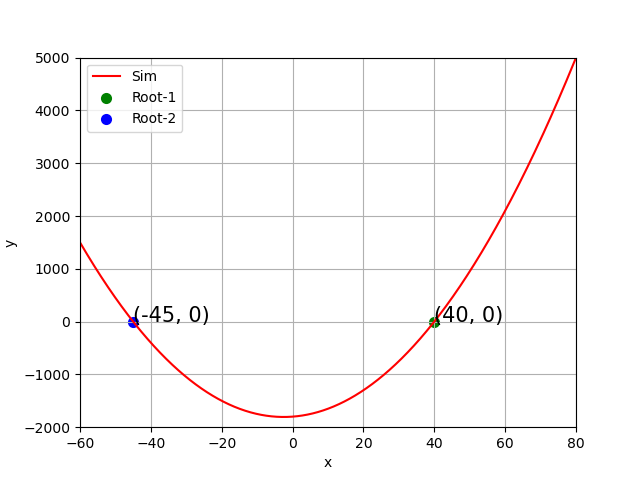
\includegraphics[width=1\columnwidth]{figs/simulated.png}
		\caption{Plot of $s^2 + 5s = 1800$}
		\label{stemplot}
	\end{figure}
\end{frame}
\end{document}
